%%%%% Point Pillar Lidar Deep Learning Face Finding %%%%%%
%%%%% Karissa Stisser, Zach Larson, Naseem Alfaqueh, Anjali Patil, Adrian Lindsey, Omar Rizk
\documentclass{article}
\usepackage[utf8]{inputenc}
\usepackage{graphicx}

\title{Point Pillar Lidar Deep Learning Face Finding}
\author{Karissa Stisser, Zach Larson, Naseem Alfaqueh\\
\\Anjali Patil, Adrian Lindsey, Omar Rizk }
\date{April 2021- https://github.com/kstisser/DeepLearningPointCloud}

\begin{document}

\maketitle

\section{Introduction}
We have created a system that uses deep learning to recognize a face in point cloud data using time series data in real time for surgical applications. As this use case is very specific, we focused on leveraging knowledge of the space and procedure to optimize the output rather than try to create a solution for all scenarios. We build a preprocessing pipeline that eliminated unnecessary points, leveraged the point pillars deep learning architecture\cite{pointpillars}, and modified the output for a point by point decision on whether that pixel belonged to the face. Development was done in two stages. First, separate pieces were developed in Jupyter notebooks. Second those notebooks were integrated into the final product. Many but not all components made it to the second stage. 
\section{Data Augmentation}
As we started with 7 point clouds, we developed a data augmentation plan to be used on both the train and test data that involves background mixing, translation, rotation, scaling, and flipping as we would like the trained algorithm to be more robust to camera placement in relation to the face. We only modified in the x and y directions, as modifications in the z directions would actually add and remove points, which we weren't confident in accurately augmenting. 

We start by matching each face with each other background points. If we have n point clouds, this creates an additional n choose 2 combination of point clouds. 
For each of these background mixed point clouds we added translation in a spiral format starting from the face center and moving outwards in 30 different locations. We continually increment the angle by 4 * pi/30 to ensure two spiral loops, and use the following equation for center face placement:
\[rt = e^{0.306*angle}\]
\[x = rt * cos(angle) + originalX\]
\[y = rt * sin(angle) + originalY\]
At each different translation we are rotating the face 10 times in addition to the original, which we consider 0 degrees, and we evenly space the other 10 between 0 and 360. We are scaling at ${2\%}$, ${4\%}$, and ${6\%}$, both bigger and smaller to make an additional 6 point clouds, keeping the face a reasonable size within the anticipated space. Because we are using random downsampling the space between the points at these scales are not a concern as it is possible we would randomly increase or decrease the scaling of the proximity of points. 
Finally, we flopped the face in each of the scaled point clouds, doubling the final count, which is:
\[
    3600 * \frac{n!}{2!(n-2)!} + n
\]
where n = the number of original point clouds. As we started with 7 point clouds, we are able to produce a total of 151,207 point clouds. As all 7 point clouds were of the same face, the next step would be to collect data of different faces with a variation on age, size, races, and distinctive features. 
\section{Data Preprocessing}
\begin{figure}[htp]
    \centering
    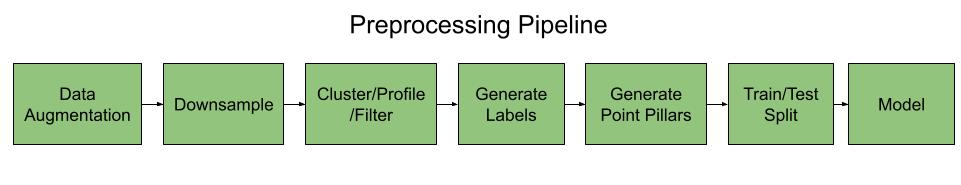
\includegraphics[scale=0.4]{PreprocessingPipeline.jpg}
    \caption{Preprocessing Pipeline}
    \label{fig:preprocessingPipeline}
\end{figure}
Because we are not able to use all points in the point cloud given due to computational speed, we chose to add preprocessing steps to eliminate unnecessary points. As this problem is meant for a specific application with specific hardware, we were able to make certain assumptions. Because we were told there will be a table or floor under the patient being operated on, we chose to begin our algorithm with a RANSAC plane finder to eliminate all points within a reasonable plane. We then randomly downsampled to 1000 points. 

Next, we developed a clustering architecture which consists of a Clusterer and Cluster Profiler. The clusterer starts by running DBSCAN with eps = 0.05 and the minimum number of samples are 10. The Cluster Profiler maintains profiles of faces using number of points in the cluster, width of the cluster, and height of the cluster. We store an ideal face (an average of our downsampled data) with 200 points, 0.1907 meters width, and 0.2487 meters height to compute a score to compare each incoming cluster against. Our score calculation is:

\[
    numPointsScore= \frac{(averageFace.numPoints - incomingFace.numPoints)}{0.5 * (maxFace.numPoints - minFace.numPoints)}
\]
\[
    widthScore= \frac{(averageFace.width - incomingFace.width)}{0.5 * (maxFace.width - minFace.width)}
\]
\[
    heightScore= \frac{(averageFace.height - incomingFace.height)}{0.5 * (maxFace.height - minFace.height)}
\]
\[
    score = numPointsScore + widthScore + heightScore
\]

We also maintain a profile for a minimum face with 100 points, 0.1 meters width, and 0.2 meters height, and a maximum face with 300 points, 0.4 meters width, and 0.6 meters height. If the incoming cluster has any value lower than the minimum face or larger than the maximum face it is given a score of -1 and is eliminated. If the cluster is not eliminated by this, its score is computed when compared to the average face, and if the score is above the threshold 0.7, it is kept for further parallel evaluation in the Machine Learning pipeline. 

\begin{figure}[htp]
    \centering
    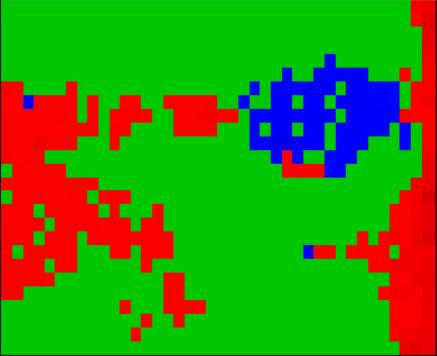
\includegraphics[scale=0.8]{pointPillars.png}
    \caption{PointPillars}
    \label{fig:pointPillars}
\end{figure}
While the clustering seems to be working well, the parameters don't seem consistent enough yet to send each cluster through the model, which was our goal. So, we are currently sending one large cluster of all data through an embedding to become a point pillar\cite{pointpillars}. However, we are using 8 feature variables, not including the reflectance value as it is not available. These pillars are formed by projecting all points in the point cloud onto the x-y plane and binning them with a simple grid. The arithmetic mean of the x, y, z values of the points in each bin are taken, as well as the x and y offset of each point from the center of the pillar (the mean values). These statistics are then combined with the three dimensional coordinates of each point to give an eight dimensional vector for each point. Once processed into point pillars, we normalize the data to be between 0 and 1 before sending it through the deep learning model. The labels also need to be processed to contain a 1 or 0 for each pillar to match in dimensions. Something that was interesting and highlighted when visualizing the point pillars were that about half of them had at least one noisy label away from the face, as shown in figure \ref{fig:pointPillars} where the blue is a pillar with a face label, the red is a pillar which have only non-face points, and the green are empty pillars. This highlights that mislabelled data being fed into the model is accentuated. 

\section{Architecture}
Once the data has been preprocessed, a vector of downsampled, clustered, point pillars are ready to enter the deep learning network. As we are working with 1200 pillars, 20 maximum points per pillar, and 8 features, the incoming shape of the data is (number of samples, 1200, 20, 8). We struggled with our model, as we failed to run due to resource constraints in a Jupyter notebook with and without TPU/GPU, locally, and with several cloud instances. Finally, with reducing to 1 batch, reducing the max points per pillar to 20, which was closer to the max points, and simplifying the model with fewer layers we were able to run locally. This resulted in the following model summary:
\begin{figure}[htp]
    \centering
    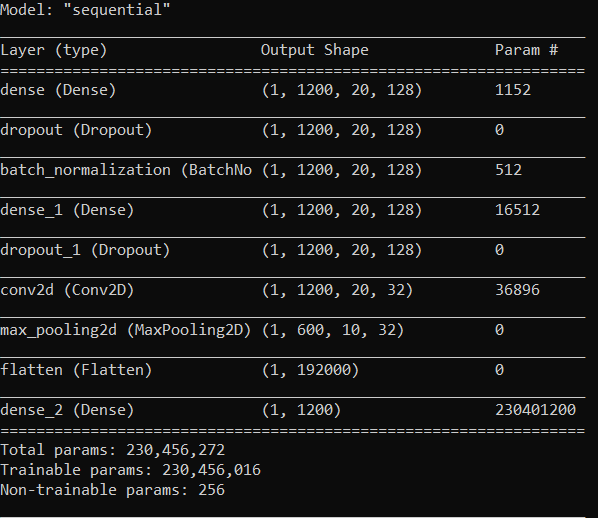
\includegraphics[scale=0.8]{model2.png}
    \caption{Model Summary}
    \label{fig:modelSummary}
\end{figure}
We compiled with an Adam optimizer with a learning rate of 0.0001 and a Binary Crossentropy loss function. We then need to remap that to the point pillars that were fed in before delivering the result. 
\section{Training}
We implement the traditional 80/20 train-test split in dividing the pre-processed data. The training and test data is treated by the point pillar method and the training data is passed to the model. The labels are per pillar where a pillar that includes at least one face point (1) or a pillar that includes no face points (0). Initially we were achieving a low accuracy of 0.2, but were able to increase the accuracy by reducing the learning rate to 0.0001. We also added he{\_}normal initialization weights to the first Dense layer to try to help overcome the problem of vanishing gradients. We analyzed what labels were being labelled incorrectly. For instance, for one face, 75{\%} of the missed labels were incorrectly labelling face labels no-face labels, and another face had 45{\%} face points being labelled incorrectly. This tells me that although we were getting 73{\%} accuracy, much more work needs to be done to improve focusing on the face being labelled accurately.  
\section{Conclusion}
While there are far too many points in a point cloud to process all points in real time, we developed a method to smartly eliminate points through RANSAC, cluster elimination, and downsampling. We developed a simple but efficient model that can achieve an accuracy of 0.73 in labeling each point as a face in the incoming point cloud. Significant speedup is necessary but possible for this system to be able to run in real time. We also have future ideas for kalman filter tracking on the face cluster to predict the location of the face in the next frame, as a face can only move a certain distance at a certain time frame. If the kalman filter has an accurate enough prediction, we will be able to eliminate all points outside of a bounding box barely larger than any head to significantly reduce the number of unnecessary points prior to running the data through the model. 
\begin{thebibliography}{9}
\bibitem{pointpillars} 
PointPillars: Fast Encoders for Object Detection from Point Clouds, Dec 14, 2018
\\\texttt{arXiv:1812.05784}
\bibitem{githubrepo}
Point Pillars in TensorFlow (2020), GitHub, https://github.com/tyagi-iiitv/PointPillars
\end{thebibliography}
\end{document}
